\documentclass[12pt]{article}
 
\usepackage[margin=1in]{geometry} 
\usepackage{amsmath,amsthm,amssymb,amsfonts}
\usepackage{color}
\usepackage{graphicx}
\graphicspath{ {Images/} }
\usepackage{float}
\setlength{\parskip}{1em}
\usepackage{cancel}
\usepackage{longtable}
\usepackage{algorithm}
\usepackage{pgf,tikz,pgfplots}
\pgfplotsset{compat=1.15}
\usepackage{mathrsfs}
\usetikzlibrary{arrows}
\pagestyle{empty}
\begin{document}

\title{Introduction to Optimisation: Project}
\author{}
\date{}
\maketitle

This repository was created as a final project for the subject ELEN90026 Introduction to Optimisation at The University of Melbourne.

The purpose of this project is to demonstrate two aspects of using the method of dual decomposition for solving an optimisation problem with a separable cost function (and one complicating variable). The first aspect is the application of parallel computing to simulate decomposing the separable problem into subproblems and solving those subproblems in parallel on separate machines. The second aspect is the affect of a limit on the packet size of messages passed between these parallel processes/machines on convergence of the overall algorithm.

In terms of hardware, the examples and results were generated using a 2.90GHz Intel i7-7500U CPU with 2 cores (4 logical processors).

\section*{Background}

\subsection*{Separable Cost Function}
In general, the analysis below is not limited to cost functions that are separated into only two parts. But for now, let's begin by dealing with this type of problem first.

The following separable unconstrained problem will be considered:
\begin{align*}
\min_{x_1,x_2,x_3}f_1(x_1,x_3)+f_2(x_2,x_3)
\end{align*}
or equivalently
\begin{align*}
\min_{x_1,\xi_1,x_2,\xi_2}\qquad&f_1(x_1,\xi_1)+f_2(x_2,\xi_2)\\
s.t.\qquad&\xi_1=\xi_2,
\end{align*}
where $x_1\in\mathbb{R}^n$, $x_2\in\mathbb{R}^m$ and $x_3,\xi_1,\xi_2\in\mathbb{R}$ for some $n$ and $m$.

\subsection*{Dual Decomposition and the Subgradient Method}
The dual function is then
\begin{align*}
q(\lambda)&=\inf_{x_1,\xi_1,x_2,\xi_2}[f_1(x_1,\xi_1)+f_2(x_2,\xi_2)-\lambda^\top(\xi_1-\xi_2)]\\
&=\inf_{x_1,\xi_1}[f_1(x_1,\xi_1)-\lambda^\top(\xi_1)]+\inf_{x_2,\xi_2}[f_2(x_2,\xi_2)+\lambda^\top(\xi_2)]\\
&=q_1(\lambda)+q_2(\lambda)
\end{align*}
We seek a $\lambda$ that maximises this dual function, which can be found using the subgradient method. Here the negative subgradient of the dual function at a given point $\lambda_k$ is given as $g_k=\xi_1-\xi_2$. The subgradient method involves iteratively
\begin{itemize}
	\item finding $(x_1,\xi_1,x_2,\xi_2)\in\arg\min\limits_{x_1,\xi_1,x_2,\xi_2}[f_1(x_1,\xi_1)+f_2(x_2,\xi_2)-\lambda^\top(\xi_1-\xi_2)]$, and
	\item updating $\lambda_{k+1}=\lambda_k-\alpha_k(\xi_1-\xi_2)$, where $\alpha_k$ is the step size.
\end{itemize}

The method of dual decomposition is simply making use of the fact that the dual function can be decomposed into $q_1(\lambda)$ and $q_2(\lambda)$ as shown above, and so finding

$(x_1,\xi_1,x_2,\xi_2)\in\arg\min\limits_{x_1,\xi_1,x_2,\xi_2}[f_1(x_1,\xi_1)+f_2(x_2,\xi_2)-\lambda^\top(\xi_1-\xi_2)]$

\noindent can instead be done by two individual agents separately finding the minimisers

$(x_1,\xi_1)\in\arg\min_{x_1,\xi_1}[f_1(x_1,\xi_1)-\lambda^\top(\xi_1)]$

$(x_2,\xi_2)\in\arg\min_{x_2,\xi_2}[f_2(x_2,\xi_2)+\lambda^\top(\xi_2)]$

\subsection*{Parallel Computing}

The \textbf{multiprocessing} module on Python was used to execute processes in parallel. A key point is that to simulate different agents separately executing tasks, this is better reflected by spawning parallel processes rather than threads.

\section*{Outcomes}

Some expected outcomes/results from this project which will be demonstrated using by the example problems:

\begin{enumerate}
	\item As a result of dual decomposition, there are steps in the subgradient method that can be done in parallel, namely finding the minimisers of the decomposed dual function. The first expectation is that parallelising these processes will not affect the convergence of the subgradient method.
	\item There is some computational overhead in spawning processes on Python. If the processes are simple computations, then serial computing may end up being faster than parallel computing due to this overhead.
	\item The number of separations in the cost function do not matter, only that individually, each separation of the function is convex.
	\item Parallel processing makes use of the multiple cores of a processor. Using a CPU with more cores means more processes can be run in parallel.
	\item The floating point precision of messages passed between agents affects the convergence of the subgradient method. We lose convergence guarantees if the messages become too imprecise.
\end{enumerate}

\section*{Problem 1}

This is a pedagogical toy problem. It is designed to show how Process and Pipe objects from the multiprocessing module on Python can be used in a separable optimisation problem. This problem relates to outcome 2, but also touches briefly on outcomes 1 and 3.

Let's use a specific example of a problem with cost function that can be partitioned into two parts. The following is the separable unconstrained optimisation problem to be solved:
\begin{align*}
\min_{x_1,x_2,x_3}\qquad& x_1^2+x_2^2+2x_3^2,
\end{align*}
where $x_1,x_2,x_3\in\mathbb{R}$. Let $x_1$ and $x_2$ both be private variables, i.e., they can only be accessed by Agent 1 and Agent 2 respectively. Let $x_3$ be a shared or public variable that can be accessed by all agents. The minimiser of this problem is obviously $(x_1^*,x_2^*,x_3^*)=(0,0,0)$, but remember, the point of this problem is really to give Python's multiprocessing module a test run on an optimisation problem. 

By applying a change of variables, the cost function can be separated and the new formulation of the problem will be
\begin{align*}
\min_{x_1,\xi_1,x_2,\xi_2}\qquad& [x_1^2+\xi_1^2]+[x_2^2+\xi_2^2]\\
s.t.\qquad&\xi_1=\xi_2,
\end{align*}
where $x_1,\xi_1,x_2,\xi_2\in\mathbb{R}$. The dual function will then be
\begin{align*}
q(\lambda)&=q_1(\lambda)+q_2(\lambda)\\
&=\inf_{x_1,\xi_1}[x_1^2+\xi_1^2-\lambda\xi_1]+\inf_{x_2,\xi_2}[x_2^2+\xi_2^2+\lambda\xi_2].
\end{align*}
The minimisers of $[x_1^2+\xi_1^2-\lambda\xi_1]$ and $[x_2^2+\xi_2^2+\lambda\xi_2]$ will be $(x_1^*,\xi_1^*)=(0,\lambda/2)$ and $(x_2^*,\xi_2^*)=(0,-\lambda/2)$ respectively. The algorithm will be as follows:

\begin{itemize}
	\item At step $k=0$, some master processor chooses an initial $\lambda(0)=1.0$ and sends $\lambda(0)$ to Agents 1 and 2. Agent 1 calculates $\xi_1^*(0)=\lambda(0)/2$, while (in parallel) Agent 2 calculates $\xi_2^*(0)=-\lambda(0)/2$. Agents 1 and 2 send $\xi_1^*(0)$ and $\xi_2^*(0)$ back to the master processor.
	\item At step $k=1$, the master processor updates $\lambda(1)=\lambda(0)-\alpha(\xi_1^*(0)-\xi_2^*(0))$ and sends $\lambda(1)$ to Agents 1 and 2. Agent 1 calculates $\xi_1^*(1)=\lambda(1)/2$, while (in parallel) Agent 2 calculates $\xi_2^*(1)=-\lambda(1)/2$. Agents 1 and 2 send $\xi_1^*(1)$ and $\xi_2^*(1)$ back to the master processor.
	\item Keep looping until $\xi_1^*(k)-\xi_2^*(k)$ is small enough, or we reach some chosen maximum number of iterations.
\end{itemize}


\subsection*{Computational Overhead}

There is some computational overhead to spawn a Process on Python. The parallel processes in this problem are computationally cheap compared to this overhead; Agent 1 just needs to compute $\xi_1^*(k)=\lambda(k)/2$ while Agent 2 only needs to compute $\xi_2^*(k)=-\lambda(k)/2$ each iteration. Thus, it is faster to just carry out the processes in series.

As a sanity check, let's simulate a more ``difficult'' problem, where the minimisers $\xi_1^*(k)$ and $\xi_2^*(k)$ may be more computationally expensive to compute. This can be done by introducing a for-loop that in the parallel processes so that on top of calculating $\xi_1^*(k)$ and $\xi_2^*(k)$, the agents must also loop through a large ``dummy'' calculation. When the ``dummy'' for-loop is made large enough (of the order $1000000$ iterations), we start to see the serial method overtake the parallel method in terms of completion time.

\begin{figure}[H]
	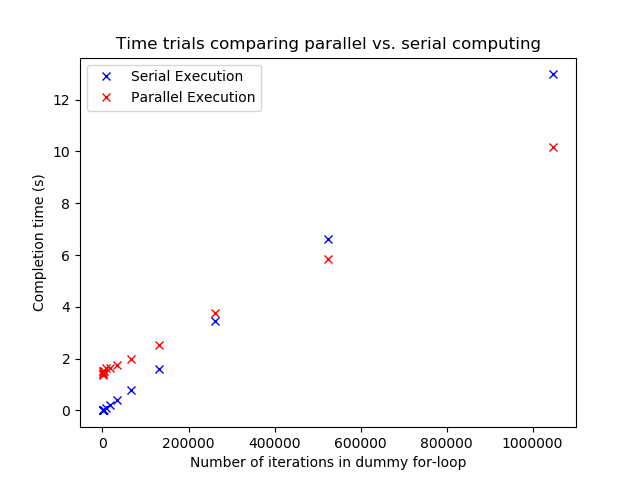
\includegraphics[scale=1]{Problem1-TimeTrial.png}
\end{figure}

Thus, we passed the sanity check. For parallel computing to finish faster than serial computing, the cost of computation per process must be larger the computational cost of spawning that process. In terms of our optimisation problem, the decomposed dual function must be decomposed into smaller functions whose minimisers are found through sufficiently complex computations, in order to observe any fruitful results from using parallel computing.

\subsection*{Convergence of Algorithm}

We get convergence to $(x_1^*,x_2^*,x_3^*)=(0,0,0)$ as expected. It turns out that convergence occurs regardless of how the variable $x_3^2$ in the cost function is separated. Given $f=x_1^2+x_2^2+2x_3^2$, convergence occurs for $f=[x_1^2+2ax_3^2]+[x_2^2+2(1-a)x_3^2]$ for all $a\in(0,1)$. This will be observed in more detail, in Problem 2.

\begin{figure}[H]
	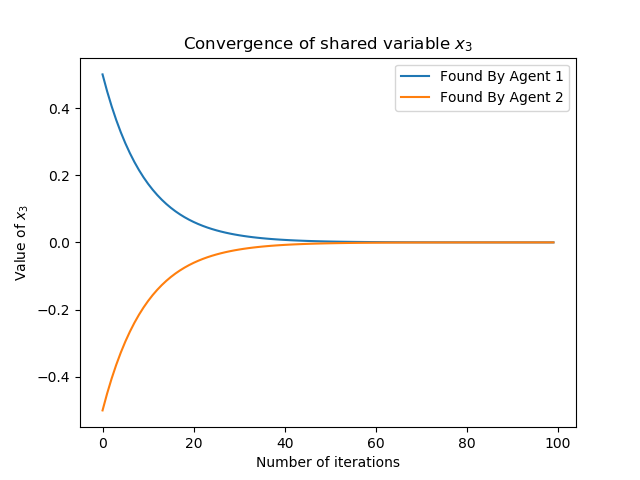
\includegraphics[scale=1]{Problem1-Convergence.png}
\end{figure}

\subsection*{How to Run}

\subsubsection*{The above examples}

Make sure you are in the correct directory. Then to run the test that generated the above plots, execute the \textbf{main.py} file, i.e. use the command

\noindent \textbf{$>>>$python main.py}

\subsubsection*{Function Descriptions}

The function \textbf{parallel.do\_parallel}, description.

Syntax: do\_parallel(max\_iter,alpha,size\_problem=0,verbose=False)

Parameter values:
\begin{itemize}
	\item max\_iter, Required. Number of iterations for the subgradient method.
	\item alpha, Required. Step size for the subgradient method.
	\item size\_problem, Default 0. Number of iterations for the dummy for-loop.
	\item verbose, Default False. Print results to screen.
\end{itemize}

Outputs:
\begin{itemize}
	\item Output 1. List containing $\xi_1^*$ for all iterations of the subgradient method.
	\item Output 2. List containing $\xi_2^*$ for all iterations of the subgradient method.
	\item Output 3. Completion time.
\end{itemize}

\subsection*{Closing Discussion for Problem 1}

This simple problem provides a framework on using the Python \textbf{multiprocessing} module, which we can carry forward to the next problem. The expected computational overhead in spawning processes has been demonstrated. As expected, the parallel processing scheme is faster than the serial processing one only for proceses with large enough complexity. And as expected, processing the minimisers of the decomposed dual function does not affect convergence to the solution of the original primal problem.

\section*{Problem 2}

Let's now observe the same results as Problem 1, but for a multidimensional problem. Consider a (convex) quadratic cost function, simply because we can write out the equation for its minimiser explicitly. In general, outcome 1 can be shown for any problem where agents act as oracles and provide the minimiser to the decomposed dual function when queried. In this problem with quadratic costs, the functions are differentiable and their gradients are linear, which makes for an easy demonstration.

\subsection*{An Example Quadratic Problem}

The following is the separable unconstrained optimisation problem to be solved:
\begin{align*}
\min_{x,y,z}\qquad& f_1(x,z)+f_2(y,z),
\end{align*}
where $x\in\mathbb{R}^n$, $y\in\mathbb{R}^m$, $z\in\mathbb{R}$ and $f_1$ and $f_2$ are quadratic in $n+1$ and $m+1$ variables respectively. In other words, the function $f_1$ has the form $f_1=\sum\limits_{i=1}^n \sum\limits_{j=i}^n \alpha_{ij}x_ix_j + \sum\limits_{i=1}^n \beta_ix_i+\gamma+\sum\limits_{i=1}^n \delta_izx_i+\epsilon z+\zeta z^2$, for some coefficients $\alpha_{ij},\beta_i,\gamma,\delta_i,\epsilon,\zeta$. The function $f_2$ can be similarly defined, $f_2=\sum\limits_{i=1}^m \sum\limits_{j=i}^m \omega_{ij}x_ix_j + \sum\limits_{i=1}^m \psi_ix_i+\phi+\sum\limits_{i=1}^m \tau_izx_i+\sigma z+\mu z^2$, for some coefficients $\omega_{ij},\psi_i,\phi,\tau_i,\sigma,\mu$.

Once again, $z$ is a shared variable that can be accessed by all agents, while $x$ and $y$ are both vectors of private variables that can only be accessed by Agent 1 and Agent 2 respectively.

By applying a change of variables, the cost function can be separated and the new formulation of the problem will be
\begin{align*}
\min_{x,\xi_1,y,\xi_2}\qquad& f_1(x,\xi_1)+f_2(y,\xi_2)\\
s.t.\qquad&\xi_1=\xi_2.
\end{align*}
The dual function will then be
\begin{align*}
q(\lambda)&=q_1(\lambda)+q_2(\lambda)\\
&=\inf_{x,\xi_1}[f_1(x,\xi_1)-\lambda\xi_1]+\inf_{y,\xi_2}[f_2(y,\xi_2)+\lambda\xi_2].
\end{align*}
The minimisers can be found by finding the gradients and setting to zero, as follows:
\begin{align*}
\nabla [f_1(x,\xi_1)-\lambda\xi_1]&=\begin{bmatrix}2\alpha_{11}x_1+\sum\limits_{i\neq1} \alpha_{1i}x_i+\beta_1+\delta_1\xi_1\\ \vdots\\ 2\alpha_{nn}x_n+\sum\limits_{i\neq n} \alpha_{ni}x_n+\beta_n+\delta_n\xi_1\\2\zeta\xi_1+(\epsilon-\lambda)+\sum\limits_{i=1}^n \delta_ix_i\end{bmatrix}\\
&=\underbrace{\begin{bmatrix}2\alpha_{11}&...&&\alpha_{1n}&\delta_1\\&& \vdots\\ \alpha_{1n}&...&&2\alpha_{nn}&\delta_n\\\delta_1&...&&\delta_n&2\zeta\end{bmatrix}}_{A_1} \underbrace{\begin{bmatrix}x_1\\ \vdots\\ x_n\\\xi_1\end{bmatrix}}_{v_1}+\underbrace{\begin{bmatrix}\beta_1\\ \vdots\\ \beta_n\\(\epsilon-\lambda)\end{bmatrix}}_{B_1}=\textbf{0}
\end{align*}
\begin{align*}
\nabla [f_2(y,\xi_2)+\lambda\xi_2]&=\begin{bmatrix}2\mu\xi_2+(\sigma+\lambda)+\sum\limits_{i=1}^m \tau_iy_i\\2\omega_{11}y_1+\sum\limits_{i\neq1} \omega_{1i}y_i+\psi_1+\tau_1\xi_2\\ \vdots\\ 2\omega_{mm}x_m+\sum\limits_{i\neq m} \psi_{mi}y_m+\omega_m+\tau_m\xi_2\end{bmatrix}\\
&=\underbrace{\begin{bmatrix}2\mu&\tau_1&...&&\tau_m\\ \tau_1&2\omega_{11}&...&&\omega_{1m}\\&&\vdots\\ \tau_m&\omega_{1m}&...&&2\omega_{mm}\end{bmatrix}}_{A_2} \underbrace{\begin{bmatrix}\xi_2\\y_1\\ \vdots\\ y_m\end{bmatrix}}_{v_2}+\underbrace{\begin{bmatrix}(\sigma+\lambda)\\\psi_1\\ \vdots\\ \psi_m\end{bmatrix}}_{B_2}=\textbf{0}
\end{align*}
The minimiser of $[f_1(x,\xi_1)-\lambda\xi_1]$ is then the solution to the set of $n+1$ linear equations and the minimiser of $[f_2(y,\xi_2)+\lambda\xi_2]$ is the solution to the set of $m+1$ linear equations above. Note, the matrices $A_1$  and $A_2$ are symmetric and must be invertible, i.e., their eigenvalues must be strictly positive; the problem is ill-conditioned if the eigenvalues are close to zero.

The same method of using the subgradient and dual decomposition from Problem 1 now applies to this problem.
\begin{itemize}
	\item At step $k=0$, some master processor chooses an initial $\lambda(0)=1.0$ and sends $\lambda(0)$ to Agents 1 and 2. Agent 1 solves $A_1v_1(0)+B_1(0)=0$ for $v_1(0)$, while (in parallel) Agent 2 solves $A_2v_2(0)+B_2(0)=0$ for $v_2(0)$. Agents 1 and 2 send $\xi_1^*(0)$ and $\xi_2^*(0)$ back to the master processor.
	\item At step $k=1$, the master processor updates $\lambda(1)=\lambda(0)-step(\xi_1^*(0)-\xi_2^*(0))$ and sends $\lambda(1)$ to Agents 1 and 2. Agent 1 solves $A_1v_1(1)+B_1(1)=0$ for $v_1(1)$, while (in parallel) Agent 2 solves $A_2v_2(1)+B_2(1)=0$ for $v_2(1)$. Agents 1 and 2 send $\xi_1^*(1)$ and $\xi_2^*(1)$ back to the master processor.
	\item Keep looping until $\xi_1^*(k)-\xi_2^*(k)$ is small enough, or we reach some chosen maximum number of iterations.
\end{itemize}

\subsection*{Combined Problem}
At this stage it is useful to observe the problem without separation of the dual function, call it the combined problem. The problem is quadratic, and the minimiser is found by finding the gradient, and ultimately solving $n+m+1$ linear equations. This means solving the problem $Av=B$, with $A$ and $B$ found by augmenting and overlapping $A_1,A_2$ and $B_1,B_2$ respectively. This is visualised below.

\begin{figure}[H]
	\centering
	\definecolor{rvwvcq}{rgb}{0.08,0.4,0.7}
	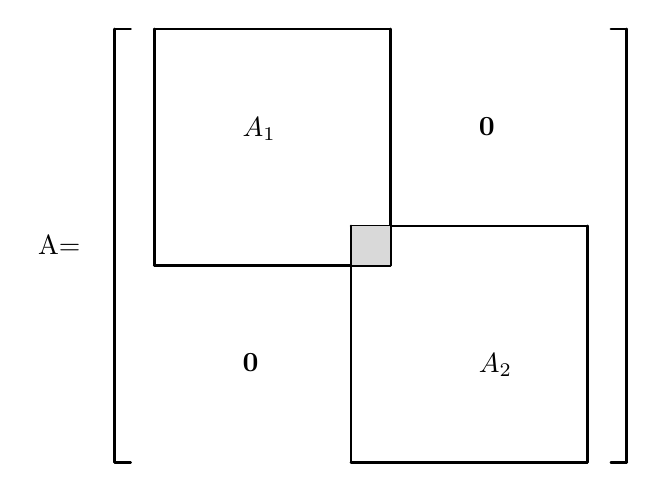
\begin{tikzpicture}[line cap=round,line join=round,>=triangle 45,x=1cm,y=1cm]
	\draw [line width=1pt] (9.5,10)-- (9.5,4.5);
	\draw [line width=1pt] (9.5,10)-- (9.7,10);
	\draw [line width=1pt] (9.7,4.5)-- (9.5,4.5);
	\draw [line width=1pt] (16,10)-- (16,4.5);
	\draw [line width=1pt] (15.8,10)-- (16,10);
	\draw [line width=1pt] (15.8,4.5)-- (16,4.5);
	\draw [line width=1pt] (10,10)-- (10,7);
	\draw [line width=1pt] (10,7)-- (13,7);
	\draw [line width=1pt] (13,7)-- (13,10);
	\draw [line width=1pt] (13,10)-- (10,10);
	\draw [line width=1pt] (12.5,7.5)-- (12.5,4.5);
	\draw [line width=1pt] (12.5,4.5)-- (15.5,4.5);
	\draw [line width=1pt] (15.5,4.5)-- (15.5,7.5);
	\draw [line width=1pt] (15.5,7.5)-- (12.5,7.5);
	\draw[fill=gray!30]    (13,7) -- (13,7.5) -- (12.5,7.5) -- (12.5,7);
	\draw (11,9) node[anchor=north west] {$A_1$};
	\draw (14,6) node[anchor=north west] {$A_2$};
	\draw (11,6) node[anchor=north west] {\textbf{0}};
	\draw (14,9) node[anchor=north west] {\textbf{0}};
	\draw (8.4,7.5) node[anchor=north west] {A=};
	\end{tikzpicture}
	\caption{Overlapping squares represent how $A_1$ and $A_2$ overlap. There is a single element in the grey overlapping region and it is equal to $2\zeta+2\mu$, the sum of the elements of $A_1$ and $A_2$ that overlap.}
\end{figure}

\begin{figure}[H]
	\centering
	\definecolor{rvwvcq}{rgb}{0.08,0.4,0.7}
	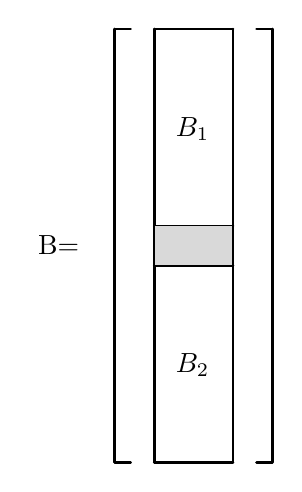
\begin{tikzpicture}[line cap=round,line join=round,>=triangle 45,x=1cm,y=1cm]
	\draw [line width=1pt] (9.5,10)-- (9.5,4.5);
	\draw [line width=1pt] (9.5,10)-- (9.7,10);
	\draw [line width=1pt] (9.7,4.5)-- (9.5,4.5);
	\draw [line width=1pt] (11.5,10)-- (11.5,4.5);
	\draw [line width=1pt] (11.3,10)-- (11.5,10);
	\draw [line width=1pt] (11.3,4.5)-- (11.5,4.5);
	\draw [line width=1pt] (10,10)-- (10,7);
	\draw [line width=1pt] (10,7)-- (11,7);
	\draw [line width=1pt] (11,7)-- (11,10);
	\draw [line width=1pt] (11,10)-- (10,10);
	\draw [line width=1pt] (10,7.5)-- (10,4.5);
	\draw [line width=1pt] (10,4.5)-- (11,4.5);
	\draw [line width=1pt] (11,4.5)-- (11,7.5);
	\draw [line width=1pt] (11,7.5)-- (10,7.5);
	\draw[fill=gray!30]    (11,7) -- (11,7.5) -- (10,7.5) -- (10,7);
	\draw (10.15,9) node[anchor=north west] {$B_1$};
	\draw (10.15,6) node[anchor=north west] {$B_2$};
	\draw (8.4,7.5) node[anchor=north west] {B=};
	\end{tikzpicture}
	\caption{Similarly, $B$ is a vector with $B_1$ and $B_2$ overlapping as shown. Only one element is in the grey overlapping region, and that element is equal to $\epsilon+\sigma$, the sum of the elements of $B_1$ and $B_2$ that overlap.}
\end{figure}
We can solve the primal problem $\min_{x,y,z} f_1(x,z)+f_2(y,z)$ directly by solving $Av+B=0$. This primal solution can be used to check convergence of solution via dual decomposition.

\subsection*{Convergence}
As a reminder, in separating the cost function, it is now a requirement that both $A_1$ and $A_2$ are well-conditioned in order to get convergence to the solution found via the combined problem. The combined matrix $A$ may be well conditioned, but depending on how $A_1$ and $A_2$ are separated, we may end up with an ill-conditioned matrices.

This picks up from where Problem 1 left off. In Problem 1, it was incorrectly concluded that convergence was still guaranteed regardless of how the shared variable $x_3^2$ was separated. It turns out that this does not hold for coefficients of $x_3^2$ that are too close to zero. If the coefficient of $x_3^2$ is too small, convergence no longer occurs. Thus, we see the key requirement that the matrices are well-conditioned appearing in Problem 1 as well.

The following plot shows convergence of the shared variable $\xi_1$ found by Agent 1 and the variable $\xi_2$ found by Agent 2 towards the actual value of $z$ found by solving $Av+B=0$ in the combined problem. Some care is taken to generate well-conditioned $A_1$ and $A_2$ matrices.

\begin{figure}[H]
	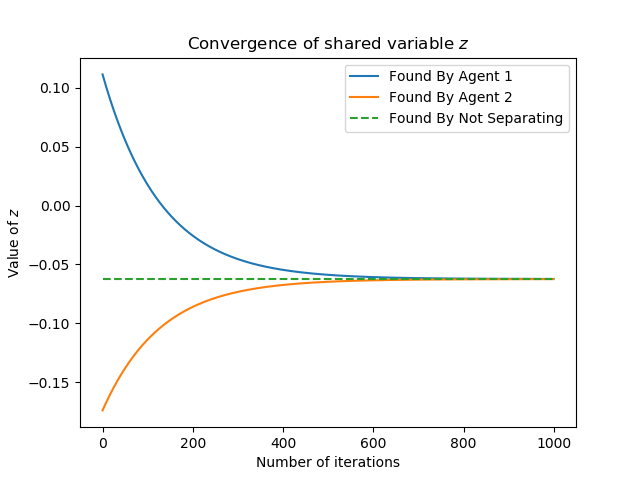
\includegraphics[scale=1]{Problem2-Convergence.png}
\end{figure}

\subsection*{Computational Overhead}

There is some computational overhead to spawn a Process on Python. Previously in Problem 1, a dummy for-loop was added to increase the complexity of each parallel process. For Problem 2, we achieve the same affect by increasing $n$ and $m$, i.e., increasing the dimensions of $A_1$ and $A_2$. The following plot shows the completion times, where the dimensions of $A_1$ and $A_2$ have been set to be equal, $n=m$.

\begin{figure}[H]
	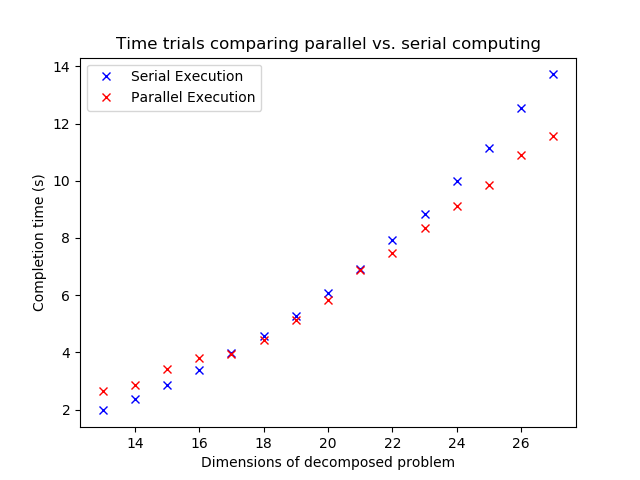
\includegraphics[scale=1]{Problem2-TimeTrial.png}
\end{figure}

In Problem 1, the completion times for both serial and parallel grew linearly with the size of the ``dummy'' for-loop. In Problem 2, the solution to $A_1x+B_1$ and $A_2x+B_2$ were found by applying Gaussian elemination, which has a complexity of order $\mathcal{O}(n^3)$. The sample plot above may not be enough to conclude cubic growth as the dimensions of the problem grow, but it can be seen that the growth is of order higher than linear growth.


\subsection*{How to Run}

\subsubsection*{The above examples}

Make sure you are in the correct directory. Then to run the test that generated the above plots, execute the \textbf{main.py} file, i.e. use the command

\noindent \textbf{$>>>$python main.py}

\subsubsection*{Function Descriptions}

The function \textbf{parallel.do\_parallel}, description.

Syntax: do\_parallel(max\_iter,alpha,A1,A2,b1,b2,verbose=False)

Parameter values:
\begin{itemize}
	\item max\_iter, Required. Number of iterations for the subgradient method.
	\item alpha, Required. Step size for the subgradient method.
	\item A1, Required. The matrix of coefficients $A_1$ as described above.
	\item A2, Required. The matrix of coefficients $A_2$ as described above.
	\item b1, Required. The matrix of coefficients $B_1$ as described above.
	\item b2, Required. The matrix of coefficients $B_2$ as described above.
	\item verbose, Default False. Print results to screen.
\end{itemize}

Outputs:
\begin{itemize}
	\item Output 1. List containing $\xi_1^*$ for all iterations of the subgradient method.
	\item Output 2. List containing $\xi_2^*$ for all iterations of the subgradient method.
	\item Output 3. Completion time.
\end{itemize}

\subsection*{Closing Discussion for Problem 2}

A quadratic problem was considered in this example, but we can extend this to any problem that can be separated into convex subfunctions. A quadratic problem was chosen because the gradient is easy to compute explicitly, but for any general problem, as long as we have access to the minimiser of each decomposition of the dual function, the analysis will hold. The order of complexity of the oracle that returns the minimisers will determine the order of growth in completion time, and the minimisers must be sufficiently computationally complex in order to see parallel processing finish faster than serial processing.

\section*{Problem 3}

Given Problem 1 and 2 both dealt with only two agents computing two processes in parallel, this presents a good opportunity to move on to a problem requiring a much larger number of agents, i.e., a demonstration of outcome 3. In addition, this problem can be used as a platform to compare the performance of hardware. As mentioned previously, the results have been generated on a 2.90GHz Intel i7-7500U CPU with 2 cores (4 logical processors). To demonstrate outcome 4, a 3.30GHz Intel i5-6600 CPU with 4 cores was used to compare against the benchmark completion times set by the i7 CPU.

Problem 3 revisits a problem from a previous assignment in this subject. It goes as follows, from the ELEN90026-Introduction to Optimisation: Homework 3 assignment brief verbatim.

\noindent\fbox{\begin{minipage}{39.5em}
		Consider a network with $n$ nodes and $m$ directed edges. Let $A$ be the incidence matrix of the network where its $ij$-th element is
		\begin{center}
			$A_{ij}=\begin{cases} 
			-1 & \text{Edge $j$ enters node $i$} \\
			1 & \text{Edge $j$ exits node $i$} \\
			0 & \text{otherwise.}
			\end{cases}$
		\end{center}
		Assume that two commodities flow through the network. Let $s_i$ and $t_i$ be the supply/demand of commodities 1 and 2 at node $i$, respectively. A positive value corresponds to supply and a negative value corresponds to demand. Let vectors $s\in\mathbb{R}^n$ and $t\in\mathbb{R}^n$ be obtained by stacking all $s_i$ and $t_i$, $i=1,...,n$. Let $f_i:\mathbb{R}^2\rightarrow \mathbb{R}$ be a convex function associated with the cost of transporting commodities 1 and 2 along edge $i$.
		
		The problem formulation:
		\begin{align*}
		\min_{x\in\mathbb{R},y\in\mathbb{R}}\qquad&\sum\limits_{i=1}^m f_i(x_i,y_i)\\
		s.t.\qquad &Ax=s,\quad Ay=t\\
		&x\geq 0,\quad y\geq0
		\end{align*}
\end{minipage}}\\\\

The cost function used in this problem will be $f_i(x_i+y_i)=(x_i+y_i)^2+0.1(x_i^2+y_i^2)$, for $i=1,...,m$. Let's allow the vectors $s$ and $t$ to be dense, they do not have to be sparse.

Now, the point of revisiting this problem is to apply parallel processing and observe an expected speed up in completion time versus serial processing. The other interesting observation we want to make here is to compare the completion times of solving this problem 2 core 2.90GHz Intel i7-7500U CPU versus running it on a 3.30GHz 4 core Intel i5-6600. But before going into that, the following describes how to obtain a solution to the optimisation problem.

In contrast to Problem 2, there are now constraint equations in the formulation, where previously Problem 2 was unconstrained. In addition, there are no shared or complicating variables in the cost function problem, it is completely separable. But the method we are going to use to solve Problem 3 will be similar to before. The dual function is
\begin{align*}
q(\alpha,\beta)&=\inf\left(\sum\limits_{i=1}^m f_i(x_i,y_i)-\alpha^\top (Ax-s)-\beta^\top(Ay-t)\right)\\
&=\alpha^\top s+\beta^\top t + \inf\left(\sum\limits_{i=1}^m f_i(x_i,y_i)-[A^\top\alpha]_ix_i-[A^\top \beta]_iy_i\right)
\end{align*}
Thus, for $i=1,...,m$, for a given $\alpha$ and $\beta$, we can let $m$ individual agents find the minimisers of $f_i(x_i,y_i)-[A^\top\alpha]_ix_i-[A^\top \beta]_iy_i$ separately, then use the subgradient to update $\alpha=\alpha-step(Ax-s)$ and $\beta=\beta-step(Ay-t)$. Note, because there are also constraints on $x,y$ being non-negative, the minimisers found by each agent must be constrained to the non-negative orthant. 


\subsection*{Convergence}

For guaranteed convergence, the graph must be connected, i.e., the incidence matrix must have rank $n-1$. Note, the chosen step size, $step$ for updating $\alpha$ and $\beta$ must decrease as $m$ increases because a larger number of columns of $A$ means more elements are being summed up when doing $Ax$ and $Ay$.

\begin{figure}[H]
	\centering
	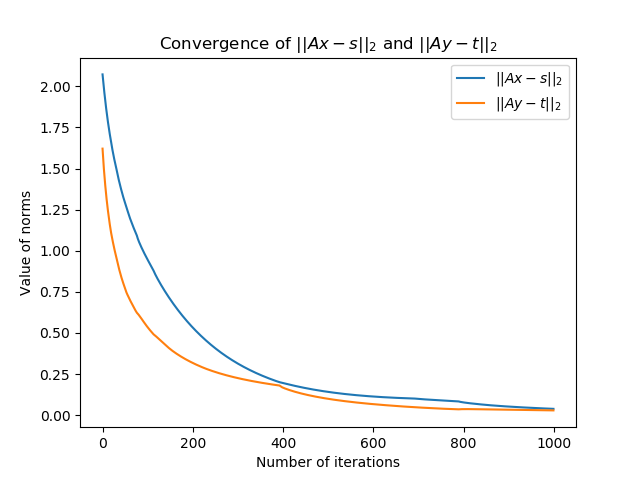
\includegraphics[scale=0.91]{Problem3-Convergence.png}
	\caption{A problem with a scale-free graph with 20 nodes.}
\end{figure}

This problem has been done in the previous assignment, so we will not dwell on convergence.

\subsection*{Computational Overhead}

For this problem, we are trying to simulate $m$ agents each computing 1 process in parallel. This is not possible with the i7 dual-core CPU that can run at most 4 processes in parallel. The closest we can get is to use the Pool object in Python's multiprocessing module and the method Pool.map. The $m$ processes are put into a pool, then offloaded to workers, which will iterate through all the tasks in the pool and compute them in parallel. With 4 logical processors, we have a maximum of 4 workers, so only 4 processes can be carried out in parallel. The following plot compares the completion time of parallelising with the Pool object versus solving the problem in series.

\begin{figure}[H]
	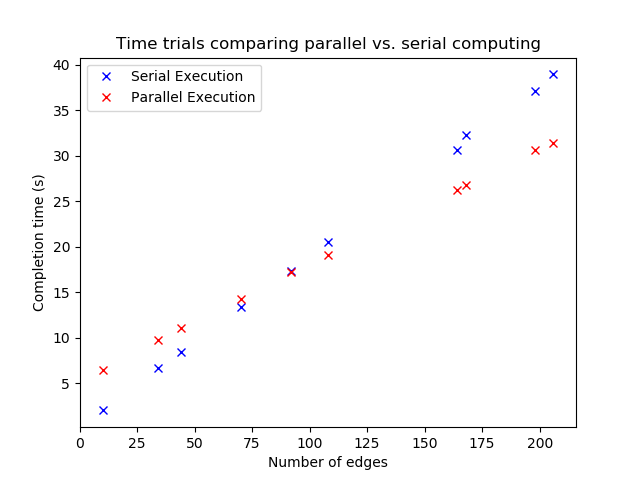
\includegraphics[scale=1]{Problem3-TimeTrial.png}
	\caption{Run on 2.90GHz Intel i7-7500U CPU with 2 cores (4 logical processors).}
\end{figure}

As expected, for a small problem size, the overhead of spawning processes in parallel means that parallel processing does worse than serial processing in terms of completion times. However, solving the problem by parallel computing becomes faster than solving via serial computing when the problem size increases. But we've seen this in Problem 1 and 2 already. It is more interesting to observe the same code run on a different machine.

\begin{figure}[H]
	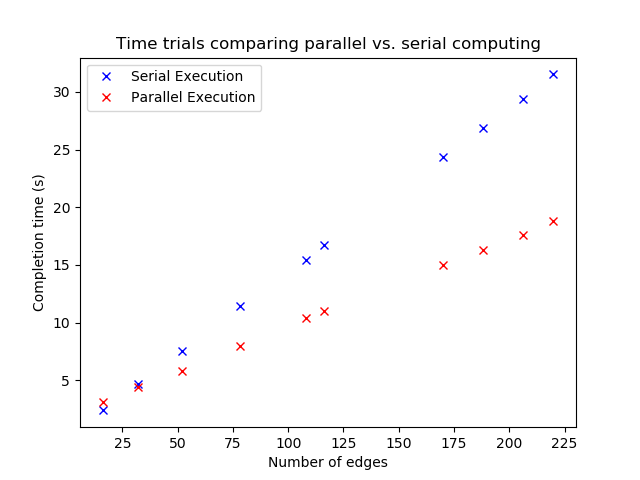
\includegraphics[scale=1]{Problem3-4cores.png}
	\caption{Run on 3.30GHz Intel i5-6600 CPU with 4 cores (4 logical processors).}
\end{figure}

The i7 is a 7th generation mobile CPU whereas the i5 is a 6th generation desktop CPU, which makes comparing them tricky. The i7 performs slightly better in terms of serial processing, but not by very much. The real benefit of having more cores in terms of parallel processing is demonstrated by the i5 solving the problem in parallel faster than the i7. So although the i7's cores are each more powerful and each core can supposedly run 2 logical processes in parallel, in reality, for the simple processes in this example problem, physically having 4 (weaker) cores solves the problem much faster.

\subsection*{How to Run}

\subsubsection*{The above examples}

Make sure you are in the correct directory. Then to run the test that generated the above plots, execute the \textbf{main.py} file, i.e. use the command

\noindent \textbf{$>>>$python main.py}

\subsubsection*{Function Descriptions}

The function \textbf{parallel.do\_parallel}, description.

Syntax: do\_parallel(max\_iter,step\_size,incidence\_matrix,s,t,verbose=False)

Parameter values:
\begin{itemize}
	\item max\_iter, Required. Number of iterations for the subgradient method.
	\item alpha, Required. Step size for the subgradient method.
	\item incidence\_matrix, Required. The incidence matrix of a connected graph as described above.
	\item s, Required. Vector of supply/demand of commodity 1 of every node. Elements of s must sum to 0.
	\item t, Required. Vector of supply/demand of commodity 2 of every node. Elements of t must sum to 0.
	\item verbose, Default False. Print results to screen.
\end{itemize}

Outputs:
\begin{itemize}
	\item Output 1. List containing $||Ax-s||_2$ for all iterations of the subgradient method.
	\item Output 2. List containing $||Ay-t||_2$ for all iterations of the subgradient method.
	\item Output 3. Completion time.
\end{itemize}

\subsection*{Closing Discussion for Problem 3}

An interesting idea that has not been pursued in this project is to increase the complexity of computing the minimisers, i.e., increase the complexity of each process. Because the cost function considered in this problem was very simple, more cores gave us faster completion time. But increasing the complexity of solving for the minimisers would be that more powerful cores may result in faster completion times than more numerous weaker cores.

\section*{Problem 4}

Let's take a look at outcome 5. We want to investigate the effect of lower precision in messages sent between agents on convergence of the subgradient method.

Revisit Problem 2, where the optimisation problem was unconstrained and had one shared variable. Recall that the dual function was given by
\begin{align*}
q(\lambda)&=q_1(\lambda)+q_2(\lambda)\\
&=\inf_{x,\xi_1}[f_1(x,\xi_1)-\lambda\xi_1]+\inf_{y,\xi_2}[f_2(y,\xi_2)+\lambda\xi_2].
\end{align*}
Dual decomposition and the subgradient method were applied to solve this problem, where we iteratively use a given $\lambda$ to solve two separate sets of linear equations, $A_1v_1=B_1$ and $A_2v_2=B_2$, and obtain $\xi_1$ and $\xi_2$, then use $\xi_1$ and $\xi_2$ to update $\lambda$.

Consider now three agents Agent 1, Agent 2 and Agent 3. Agent 3 computes the updates $\lambda=\lambda-\alpha(\xi_1-\xi_2)$, then sends $\lambda$ to both Agent 1 and 2. Agents 1 and 2 respectively solve $A_1x_1=B_1$ and $A_2x_2=B_2$, then send $\xi_1$ and $\xi_2$ to Agent 3. This is repeated for some specified number of iterations. The figure below shows one iteration of this.

\begin{figure}[H]
	\centering
	\definecolor{rvwvcq}{rgb}{0.08,0.4,0.7}
	\begin{tikzpicture}[line cap=round,line join=round,>=triangle 45,x=1cm,y=1cm]
	\draw [line width=1pt] (-8,4) circle (0.7cm);
	\draw [line width=1pt] (-3,4) circle (0.7cm);
	\draw (-10.5,5.5) node[anchor=north west] {1) Agent 3: Updates $\lambda$};
	\draw [line width=1pt] (-7,4.5)-- (-4,4.5);
	\draw [line width=1pt] (-4,4)-- (-7,4);
	\draw [line width=1pt] (-8,1) circle (0.7cm);
	\draw [line width=1pt] (-8.3,3)-- (-8.3,2);
	\draw [line width=1pt] (-7.7,2)-- (-7.7,3);
	\draw (-3.6,5.5) node[anchor=north west] {3) Agent 1: Solves $A_1x_1+B_1=0$};
	\draw (-9,0) node[anchor=north west] {3)Agent 2: Solves $A_2x_2+B_2=0$};
	\draw (-6,5.2) node[anchor=north west] {2) Send $\lambda$};
	\draw (-6,3.9) node[anchor=north west] {4) Send $\xi_1$};
	\draw (-7.5,2.7) node[anchor=north west] {4) Send $\xi_2$};
	\draw (-10.5,2.7) node[anchor=north west] {2) Send $\lambda$};
	\begin{scriptsize}
	\draw [fill=rvwvcq,shift={(-4,4.48)},rotate=270] (0,0) ++(0 pt,3.75pt) -- ++(3pt,-6pt)--++(-6.5pt,0 pt) -- ++(3pt,5.5pt);
	\draw [fill=rvwvcq,shift={(-7,4)},rotate=90] (0,0) ++(0 pt,3.75pt) -- ++(3pt,-6pt)--++(-6.5pt,0 pt) -- ++(3pt,5.5pt);
	\draw [fill=rvwvcq,shift={(-8.3,2)},rotate=180] (0,0) ++(0 pt,3.75pt) -- ++(3pt,-6pt)--++(-6.5pt,0 pt) -- ++(3pt,5.5pt);
	\draw [fill=rvwvcq,shift={(-7.7,3)},rotate=0] (0,0) ++(0 pt,3.75pt) -- ++(3pt,-6pt)--++(-6.5pt,0 pt) -- ++(3pt,5.5pt);
	\end{scriptsize}
	\end{tikzpicture}
	\caption{Steps 1, 2, 3, 4 show the procedure in a single iteration of the subgradient method.}
\end{figure}

Previously, messages were assumed to have unlimited size, i.e., there is no floating point error when $\lambda$, $\xi_1$ and $\xi_2$ are sent between Agents 1, 2 and 3. Let's now consider a limit on message size. Assume messages are sent in binary, then there is a limit on the number of bits that can be sent.

\subsection*{Word Limit}

The following terms will be used to describe a binary number.
\begin{center}
	$\underbrace{\pm}_{\text{sign}}\underbrace{10101010101010}_{\text{binary integer}}\underbrace{.}_{\text{binary point}}\underbrace{1010101010101010}_{\text{binary fraction}}$
\end{center}


For the example problems generated, it so happens that the variable $\lambda$ is in general larger than $\xi_1$ and $\xi_2$. Messages involving $\lambda$ require at least 3 binary integer bits, while messages involving $\xi_1$ and $\xi_2$ generally have a binary integer of 0, i.e., they converge to values with absolute values smaller than 1.

Let's vary the limit on the number of bits used to represent the binary fraction, and assume the number of bits used to represent the binary integer is limited to 3 bits plus 1 bit for the sign. Thus, the word limit referred to below is the limit on the number of bits used to represent the binary fraction of a message, not including the sign and integer bits.

\subsection*{Convergence}

In order to measure convergence, we need a benchmark. Recall from Problem 2 the combined problem, where $A_1$ and $A_2$ are overlapped to form $A$, and $B_1$ and $B_2$ overlapped to form $B$. The combined problem $Av+B=0$ can be solved, and we can use the vector $v$ as a benchmark to measure convergence. Let $v^*$ be the solution to the problem $Av+B=0$, let $v_1^*$ be the solution to the problem $A_1v_1+B_1=0$ and let $v_1^*$ be the solution to the problem $A_2v_2+B_2=0$. The dimensions do not match, so let's overlap $v_1^*$ and $v_2^*$

\begin{figure}[H]
	\centering
	\definecolor{rvwvcq}{rgb}{0.08,0.4,0.7}
	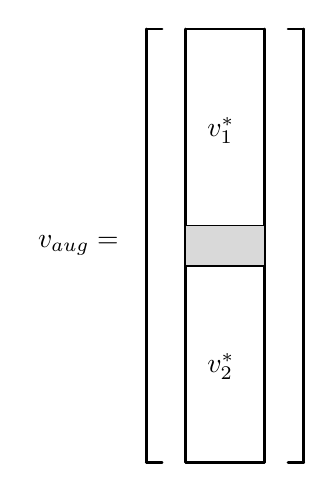
\begin{tikzpicture}[line cap=round,line join=round,>=triangle 45,x=1cm,y=1cm]
	\draw [line width=1pt] (9.5,10)-- (9.5,4.5);
	\draw [line width=1pt] (9.5,10)-- (9.7,10);
	\draw [line width=1pt] (9.7,4.5)-- (9.5,4.5);
	\draw [line width=1pt] (11.5,10)-- (11.5,4.5);
	\draw [line width=1pt] (11.3,10)-- (11.5,10);
	\draw [line width=1pt] (11.3,4.5)-- (11.5,4.5);
	\draw [line width=1pt] (10,10)-- (10,7);
	\draw [line width=1pt] (10,7)-- (11,7);
	\draw [line width=1pt] (11,7)-- (11,10);
	\draw [line width=1pt] (11,10)-- (10,10);
	\draw [line width=1pt] (10,7.5)-- (10,4.5);
	\draw [line width=1pt] (10,4.5)-- (11,4.5);
	\draw [line width=1pt] (11,4.5)-- (11,7.5);
	\draw [line width=1pt] (11,7.5)-- (10,7.5);
	\draw[fill=gray!30]    (11,7) -- (11,7.5) -- (10,7.5) -- (10,7);
	\draw (10.15,9) node[anchor=north west] {$v_1^*$};
	\draw (10.15,6) node[anchor=north west] {$v_2^*$};
	\draw (8,7.5) node[anchor=north west] {$v_{aug}=$};
	\end{tikzpicture}
	\caption{Create $v_{aug}$, a vector with $v_1^*$ and $v_2^*$ overlapping as shown. Only one element is in the grey overlapping region, and that element is equal to the \textbf{mean} of the elements of $v_1^*$ and $v_2^*$ that overlap.}
\end{figure}

Finally, our measure of convergence will be $||v_{aug}-v^*||_2$.

\begin{figure}[H]
	\centering
	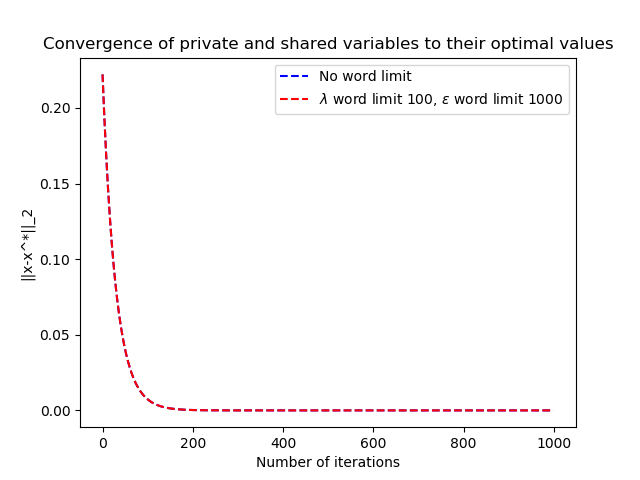
\includegraphics[scale=0.5]{Problem4-Convergence1.png}
	\caption{Large word limits.}
\end{figure}

\begin{figure}[H]
	\centering
	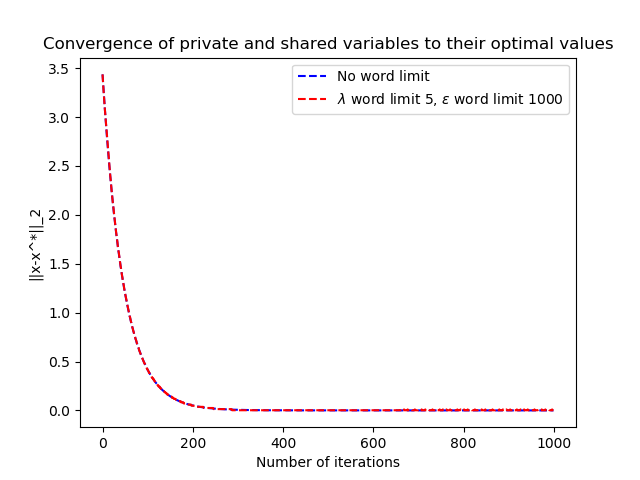
\includegraphics[scale=0.5]{Problem4-Convergence2.png}
	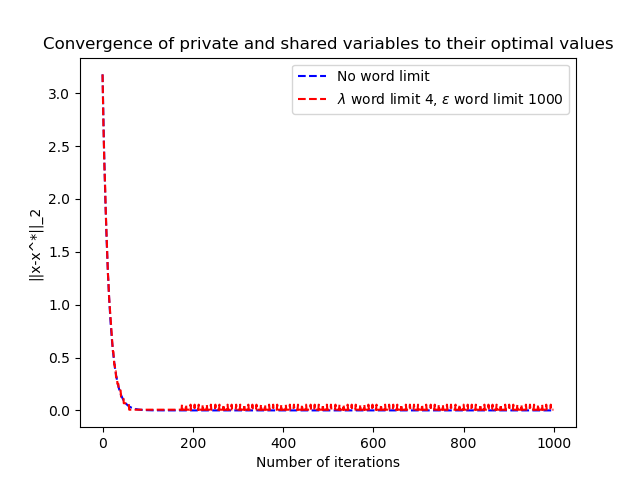
\includegraphics[scale=0.5]{Problem4-Convergence3.png}
	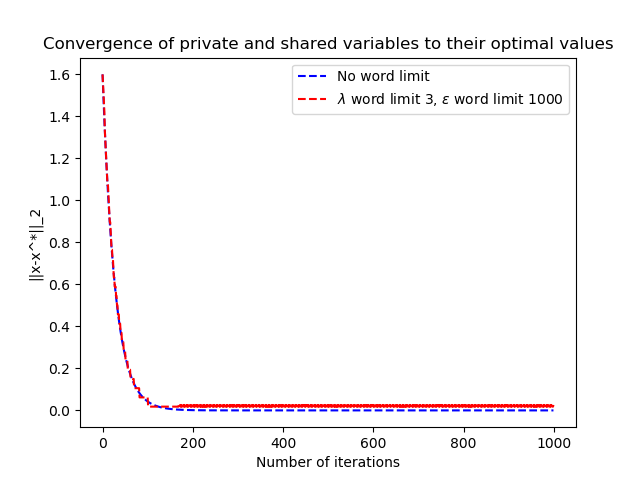
\includegraphics[scale=0.5]{Problem4-Convergence4.png}
	\caption{Decreasing the word limit on $\lambda$.}
\end{figure}

\begin{figure}[H]
	\centering
	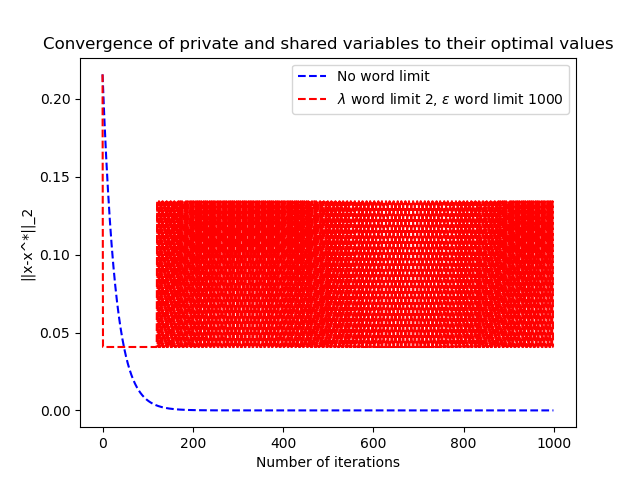
\includegraphics[scale=0.5]{Problem4-Convergence5.png}
	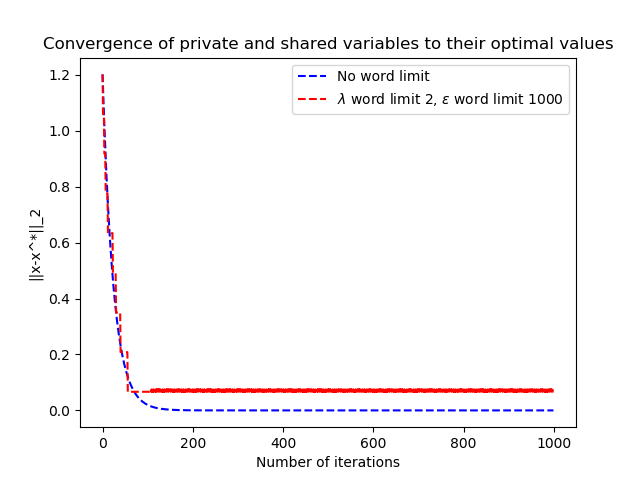
\includegraphics[scale=0.5]{Problem4-Convergence6.png}
	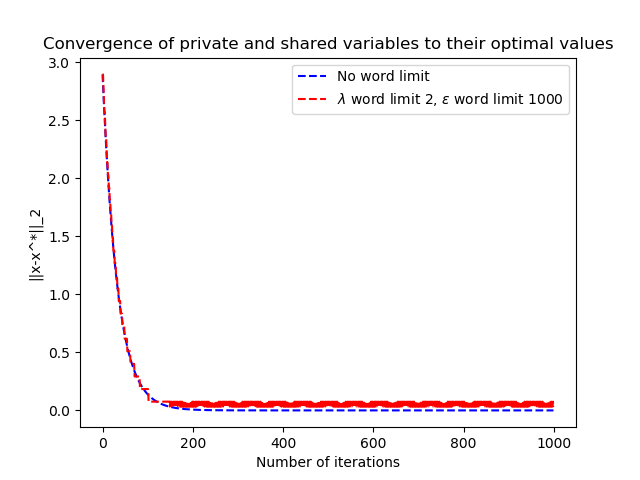
\includegraphics[scale=0.5]{Problem4-Convergence7.png}
	\caption{Convergence for a given limit on $\lambda$ is somewhat dependent on the coefficients of the problem.}
\end{figure}

For low precision on $\lambda$, we enter some limit cycle behaviour when rounding $\lambda$ to the closest limited-bit binary representation then recalculation $\xi$, and then reupdating $\lambda$, etc. In the plots below, we take a closer look at a specific problem, plotting the steady state behaviour (the last 50 iterations out of 1000) of $\lambda$. Three different $\lambda$ values are shown, $\lambda$ from the precise problem where no word limit was applied, $\lambda$ from the imprecise problem with a word limit of 3, $\lambda$ of the imprecise problem rounded down to the nearest binary number.

\begin{figure}[H]
	\centering
	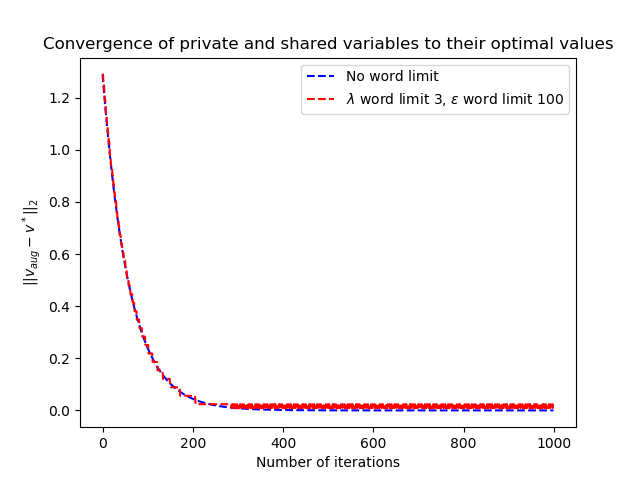
\includegraphics[scale=0.5]{Problem4-lambda1.png}
	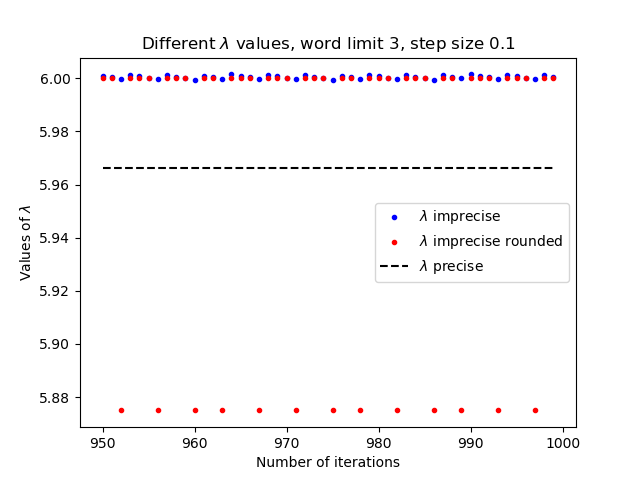
\includegraphics[scale=0.5]{Problem4-lambda2.png}
	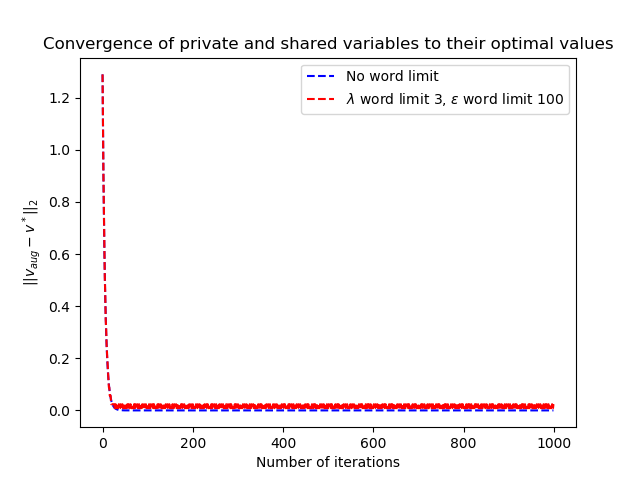
\includegraphics[scale=0.5]{Problem4-lambda3.png}
	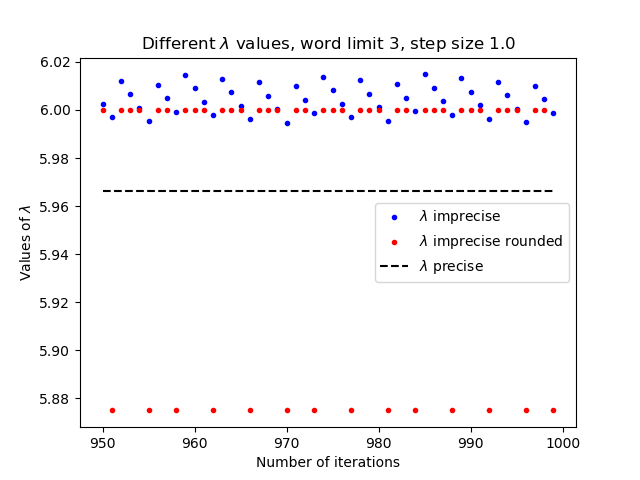
\includegraphics[scale=0.5]{Problem4-lambda4.png}
	\caption{Cyclic behaviour of $\lambda$ when its true value is 5.966, which lies beetween 6.000 and 5.875.}
\end{figure}

%Let the precise $\lambda$ be denoted $\lambda_t$ and the steady state value of $||v_{aug}-v^*||_2$ for the precise problem be $e_{true}$. Let the steady state value of $||v_{aug}-v^*||_2$ be $e_{imprecise}$. Let $v_{aug}(\lambda)$ be the result of solving $A_1v_1+B_1(\lambda)=0$ and $A_2v_2+B_2(\lambda)=0$ for a given $\lambda$ and augmenting the result (see Figure 7). Then the error bound $||e_{true}-e_{imprecise}||$ will be given by $||v_{aug}(\lambda_t+word)-v_{aug}(\lambda_t-word)||$, where $word$ is the word limit on $\lambda$.

\begin{figure}[H]
	\centering
	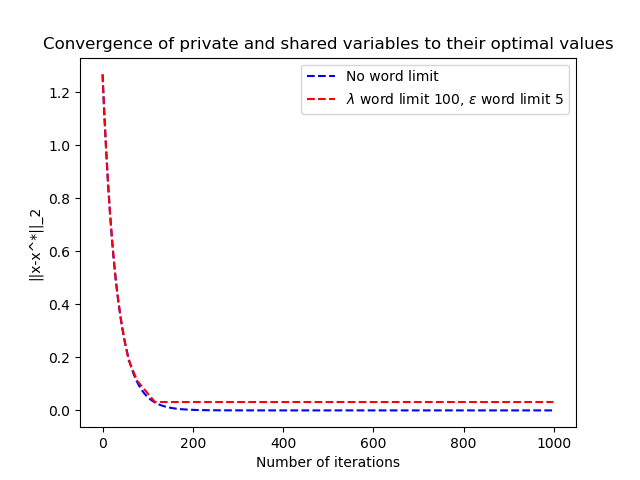
\includegraphics[scale=0.5]{Problem4-Convergence8.png}
	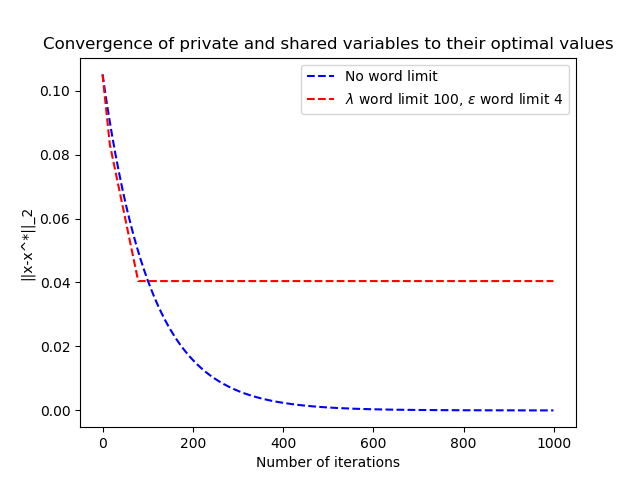
\includegraphics[scale=0.5]{Problem4-Convergence9.png}
	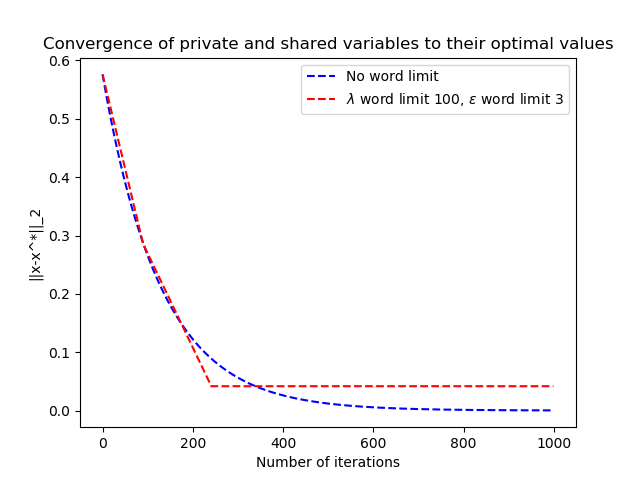
\includegraphics[scale=0.5]{Problem4-Convergence10.png}
	\caption{Similarly, convergence for a given limit on $\xi$ is also somewhat dependent on the randomly generated the problem.}
\end{figure}

With low precision on $\xi$ the error appears to be constant in steady state. Presumably in the case of low precision on $\xi$, the constant error is the rounding error caused by rounding $\xi$ to the closest limited-bit binary representation.

\subsection*{How to Run}

\subsubsection*{The above examples}

Make sure you are in the correct directory. Then to run the tests that generated the above plots, execute the \textbf{main.py} file, i.e. use the command

\noindent \textbf{$>>>$python main.py}

Vary lambda\_word\_limit and eps\_word\_limit to generate plots with different binary message limits.

\subsubsection*{Function Descriptions}

The function \textbf{conversions.float2bin}, description.

Syntax: float2bin(number, places)

Parameter values:
\begin{itemize}
	\item number, Required. A float variable that is to be converted to binary representation.
	\item places, Required. Number of bits used to represent the binary fraction of the input number. There is no limit on the number of bits used to represent the binary integer of the input number.
\end{itemize}

Outputs:
\begin{itemize}
	\item Output 1. Binary string representation of the input number. 
\end{itemize}

\noindent The function \textbf{conversions.bin2float}, description.

Syntax: bin2float(bin\_str)

Parameter values:
\begin{itemize}
	\item bin\_str, Required. A binary string representation that is to be converted to float.
\end{itemize}

Outputs:
\begin{itemize}
	\item Output 1. Float representation of input binary string. 
\end{itemize}

\noindent The function \textbf{imprecise.do\_imprecise}, description.

Syntax: do\_imprecise(max\_iter,alpha,A1,A2,b1,b2,xstar,

\qquad\qquad\qquad\qquad lambda\_word\_limit,xi\_word\_limit,verbose=False)

Parameter values:
\begin{itemize}
	\item max\_iter, Required. Number of iterations for the subgradient method.
	\item alpha, Required. Step size for the subgradient method.
	\item A1, Required. The matrix of coefficients $A_1$ as described above.
	\item A2, Required. The matrix of coefficients $A_2$ as described above.
	\item b1, Required. The matrix of coefficients $B_1$ as described above.
	\item b2, Required. The matrix of coefficients $B_2$ as described above.
	\item xstar, Required. True solution to the problem.
	\item lambda\_word\_limit, Required. Word limit of $\lambda$.
	\item xi\_word\_limit, Required. Word limit of $\xi$.
	\item verbose, Default False. Print results to screen.
\end{itemize}

Outputs:
\begin{itemize}
	\item Output 1. The measure of convergence described above, i.e., $||x_{aug}-x^*||_2$.
\end{itemize}

\end{document}